\documentclass[12pt,a4paper,dvipsnames]{article}
\usepackage{polynom}
\usepackage{amsmath}
\usepackage{tikz}
\usetikzlibrary{shapes}
\usepackage{pgfplots}
\usepackage{amssymb}
\usepackage{amsthm}
% \usepackage{utopia}
% \usepackage{venturis}
\usepackage{libertine}

% \usepackage[dvipsnames]{xcolor}
\usepackage{hyperref}
\hypersetup{
    colorlinks=true,
    linkcolor=BrickRed,
    filecolor=magenta,      
    urlcolor=cyanjj
}

\title{Correction Partiel Algèbre}
\date{\today}

\begin{document}
% Delete if you do not want a title page
{\maketitle}

% Question 1 {{{ %
\section{Egalité Ensemble}%
\label{sec:egalité_ensemble}

On cherche à démontrer par \textbf{double inclusion} l'égalité ensembliste
suivante:

\begin{equation}
    \label{eq:equa_ensemble}
    \underbrace{(A \Delta B) \cap C}_{F} = \underbrace{(A\cap C) \Delta (B\cap
    C)}_{G}
\end{equation}

\begin{enumerate}
    \item $F \subset G$
        \begin{eqnarray*}
            \text{Soit } x\in F & \implies&  x\in (A\Delta B) \text{ et }
            x\in C\\[4pt]
                                & \implies & \big[x\in (A/B) \text{ ou }
                                x\in (B/ A)\big] \text{ et } x\in C\\[4pt]
                                &\implies & \big[ x \in (A\cap C)
                                    /(B\cap C)\big] \text{ ou } \big[ x \in (B\cap C)
                                /(A\cap C)\big] \\[4pt]
                                &\implies& x \in G
        \end{eqnarray*}

    \item $G \subset F$:

        \begin{eqnarray*}
            \text{Soit } x\in G  & \implies &   x\in \big[ (A\cap C) / (B\cap
            C)\big]\text{ ou } \big[ (B\cap C) / (A\cap
    C)\big]\\[4pt]
      & \implies & x\in \big[ (A\cap C) / B\big]\text{ ou } \big[ (B\cap C) /
  A\big]\\[4pt]
  & \implies & \big[ x \in A/B \text{ ou } x \in B/A\big] \text{ et } \big[x\in
  C\big]\\
    & \implies & x\in \big[ A \Delta B\big]\\[4pt]
  & \implies & x\in F
        \end{eqnarray*}

\end{enumerate}
% }}} Question 1 %
% Question 2 {{{ %
\section{Fonction caractéristique}%
\label{sec:fonction_caractéristique}

\begin{enumerate}
    \item Fonction caractéristique de $F$:

\begin{eqnarray*}
    \pi_{F} &=& \pi_{A\Delta B}\;\pi_C\\
            &=& \big[\pi_A + \pi_B - 2\pi_A\pi_B\big]\pi_C \\
\end{eqnarray*}


\item Fonction caractéristique de $G$:

    \begin{eqnarray*}
        \pi_G & = & \pi_{A\cap C}  + \pi_{B\cap C} - 2 \pi_{A\cap B\cap C}\\
              & = & \pi_A\;\pi_C   + \pi_B\;\pi_C  -
              2\big(\pi_A\;\pi_B\big)\pi_C\\
              & = & \big[\pi_A + \pi_B -2\pi_B\pi_C\big]\pi_C
    \end{eqnarray*}
\item D'après les deux équations on conclut que :

    \begin{eqnarray*}
        \pi_F &=& \pi_G\\
              &\iff  & F = G
    \end{eqnarray*}
\end{enumerate}

% }}} Question 2 %
% Equivalence Injection Surjection {{{ %
\section{Injection/Surjection}%
\label{sec:injection_surjection}

Soit une application  $f:E\longrightarrow E$ tel que
\begin{equation}
    \label{eq:equality_injec_surj}
    f\circ f \circ f = f
\end{equation}


\begin{itemize}
    \item \textbf{Montrer que si f est injective alors elle est surjective} :

        Pour démontrer que $f$ est surjective, il faut démontrer que tout
        élément $y\in E$ admet au moins un antécédent.\\

        Soit alors $y\in E$, en utilisant l'égalité~\eqref{eq:equality_injec_surj}, on
        obtient que 
        \begin{equation}
            f\Big(f\big(f(y)\big)\Big) = f(y)
        \end{equation}

        % En utilisant l'injectivité de $f$ on conclut que
        \begin{equation}
            \label{eq:found_ant} 
            f\big(f(y)\big) = y
        \end{equation}
        Ainsi on as prouvé que $y$ admet un antécédent qui est $f(y)$.
        D'où, f est \textbf{surjective}.

    \item \textbf{Montrer que si $f$ est surjective alors elle est injective} 

\begin{proof}
  Soit deux éléments $x_1$ et $x_2$ dans $E$ tel que
  \begin{equation}
    \label{eq:equality}
    f(x_1) = f(x_2)=y
  \end{equation}
  Par absurde, supposons que $x_1 \neq x_2$, comme $f$ est surjective on as alors,

  $\exists x_1^{'}, x_2^{'}\in E$ tel que

  \begin{equation*}
    \left\{\begin{array}{l}
        x_1 = f(x_1^{'})\\[4pt]
      x_2 = f(x_2^{'})
    \end{array}
    \right.
  \end{equation*}

  On utilise maintenant le fait que $f=f\circ f \circ f$ de l'équation
  \eqref{eq:equality_injec_surj}, on aura

  \begin{equation*}
    \left\{\begin{array}{l}
        x_1 = f(f(\underbrace{f(x_1^{'})}_{x_1}))\\[10pt]
        x_2 = f(f(\underbrace{f(x_2^{'})}_{x_2}))
    \end{array}
    \right.
  \end{equation*}

  En utilisant l'égalité des images dans l'équation \eqref{eq:equality}, on aura
  \begin{equation*}
    \left\{\begin{array}{l}
        x_1 = f(\underbrace{f(x_1)}_{y}))\\[10pt]
        x_2 = f(\underbrace{f(x_2)}_{y})
    \end{array}
    \right.
  \end{equation*}

  Ainsi on aura 

  \begin{equation*}
    \left\{\begin{array}{l}
        x_1 = f(y)\\[10pt]
        x_2 = f(y)
    \end{array}
    \right.
  \end{equation*}

Aini on aura que $x_1=x_2$. Contradiction !!

\end{proof}

\end{itemize}
% }}} Equivalence Injection Surjection %
% Relation Equivalence {{{ %
\section{Relation Equivalence}%
\label{sec:relation_equivalence}

On considère dans  dans le plan $\mathbb{R}^2$, la relation 

\begin{equation}
    \label{eq:relation_equiv}
    (x_1, y_1) \mathcal{R} (x_2, y_2) \iff x_1 - 5y_2 = x_2 - 5y_1
\end{equation}

    \begin{enumerate}
        \item Montrer que $\mathcal{R}$ est une relation d'équivalence:

            \begin{description}
                \item[Réflexive]: Soit $(x_1, y_1)\in \mathbb{R}^2$,  on as $$
                    x_1 - 5y_1 = x_2 - 5y_1$$

                    On conclut que
                    $(x_1,y_1) \mathcal{R} (x_1, y_1)$.\\[4pt]

                \item [Symétrique]: Soit $P_1=(x_1, y_1)$ et $P_2=(x_2, y_2)$.
                    tel que $ P_1\;\mathcal{R}\; P_2$
                    On a alors:
                    \begin{equation}
                        x_1 - 5y_2 = x_2 - 5y1
                    \end{equation}
                    En permutant les équation on obtient que $x_2 - 5y_1 = x_1 -
                    5y_2$. Ainsi 

                    \begin{equation}
                        P_1 \; \mathcal{R} \; P_2
                    \end{equation}

                \item [Transitive] Soient $P_1(x_1,y_1)$, $P_2=(x_2, y_2)$ et
                    $P_3=(x_3,
                    y_3)$ trois points de $\mathbb{R}^2$ tel que .
                    $$
                    P_1 \mathcal{R} P_2 \text{ et } P_2 \mathcal{R} P_3
                    $$

                    On aura lors 
                    \begin{equation}
                        \left\{\begin{array}{lll} x_1 - 5y_2 &=& x_2 - 5y_1\\
                        x_2 - 5y_3 &=& x3 - 5y_2 \end{array}\right.
                    \end{equation}
                    En prenant la somme on obtient
                    \begin{equation}
                        x_1 -5y_2 + x_2 -5y_3 = x_2 -5y_1 + x_3 -5y_2
                    \end{equation}

                    qui se simplifie en 
                    \begin{equation}
                        x_1 - 5y_3 = x3 - 5y_1
                    \end{equation}

                    \begin{equation}
                        P_1\;\mathcal{R}\; P_3
                    \end{equation}

            \end{description}
        \item Dessin classe d'équivalence:
            Soit un point $P=(a,b) \in \mathbb{R}^2$.
            \begin{equation}
                \label{eq:class_equiv_q4}
                \text{Cl}(P) = \left\{ (x,y) \in \mathbb{R}^2\;|\; \underbrace{a
                + 5b}_{f(a,b)} = \underbrace{x +
        5y}_{f(x,y)}\right\}
            \end{equation}

            \begin{equation}
                \label{eq:class_equiv_q4}
                \text{Cl}(P) = \left\{ (x,y) \in \mathbb{R}^2\;|\; f(a,b) =
                f(x,y)\right\}
            \end{equation}
            Ainsi la classe $\text{Cl}(a,b)$ est l'ensemble des points qui
            ont la même image que $(a,b)$ par la fonction
            $f:(x,y)\longrightarrow x + 5y$
    \end{enumerate}

% }}} Relation Equivalence %
% Relation d'ordre {{{ %
\section{Relation d'ordre}%
\label{sec:relation_d_ordre}

Pour deux points dans $P_1, P_2 \in\mathbb{R}^2$ on considère la relation
suivante:

\begin{equation}
    \label{eq:relation_ordre}
    P_1(x1,y_1) \;\mathcal{R}\; P_2(x_2, y_2)\iff x_1 \leq x_2 \text{ et }
        y_1\leq y_2
\end{equation}

\begin{enumerate}
    \item Démontrer que c'est une relation d'ordre?
    On considère trois points $P_1(x_1, y_1), P_2(x_2, y_2)$ et $P_3=(x_3,y_3)$.
\begin{description}
    \item[Réflexive]:

        On a $ x_1 \leq x_1 \text{ et } y_1\leq y_1$ alors:
        $$  
        P_1 \;\mathcal{R}\; P_1 \quad \forall P_1\in \mathbb{R}^2
        $$

    \item[Transitive]
        On suppose que $P_1\;\mathcal{R}\; P_2$ et $P_2\;\mathcal{R}\; P_3$. On
        as alors:

        \begin{equation}
            \left\{\begin{array}{lll} x_1&\leq & x_2\\
            y_1&\leq&y_2\end{array}\right. et \left\{
\begin{array}{lll} x_2&\leq & x_3\\
            y_2&\leq&y_3\end{array}
        \right.
        \end{equation}

        On conclut alors que:
        \begin{equation}
            \begin{array}{lll} x_1&\leq & x_3\\
            y_1&\leq&y_3\end{array}
        \end{equation}
        Ainsi:
        \begin{equation}
            P_1\; \mathcal{R}\; P_3
        \end{equation}
    \item[Antisymétrique]:
        On suppose que $P_1\;\mathcal{R}\; P_2$ et $P_2\;\mathcal{R}\; P_1$. On
        as alors:

        \begin{equation}
            \left\{\begin{array}{lll} x_1&\leq & x_2\\
            y_1&\leq&y_2\end{array}\right. et \left\{
\begin{array}{lll} x_2&\leq & x_1\\
            y_2&\leq&y_1\end{array}
        \right.
        \end{equation}

        On conclut alors que:
        \begin{equation}
            \begin{array}{lll} x_1&= & x_2\\
            y_1&=&y_2\end{array}
        \end{equation}
        Ainsi:
        \begin{equation}
            \big[ P_1\;\mathcal{R}\; P_2 \text{ et }P_2\;\mathcal{R}\; P_1
            \big]\implies P_1 = P_2
        \end{equation}
\end{description}
Ainsi on conclut que $\mathcal{R}$ est une relation d'\textbf{ordre}.
\item Représenter éléments supérieures et inférieurs.
    Soit $P=(a,b)\in \mathbb{R}^2$, un point dans le plan, alors les éléments
    inférieurs à $(a,b)$ vérifient la relation suivante:

    \begin{equation}
        \label{eq:elem_inf}
         Inf_{(a,b)} =\left\{ (x,y)\in\mathbb{R}^2\;|\; (x,y)\;\mathcal{R}\;(a,b)\right\} 
    \end{equation}

    \begin{equation}
        \label{eq:elem_inf}
        Inf_{(a,b)} =\left\{ (x,y)\in\mathbb{R}^2\;|\; x\leq a\text{ et } y\leq
        b\right\} 
    \end{equation}
    De même on obtient que:

    \begin{equation}
        \label{eq:elem_sup}
        Sup_{(a,b)} =\left\{ (x,y)\in\mathbb{R}^2\;|\; x\geq a\text{ et } y\geq
        b\right\} 
    \end{equation}

    Une illustration de ces deux ensembles est présentée dans la
    (figure.\ref{fig:point_sup}).
\begin{figure}[htpb]
\begin{center}
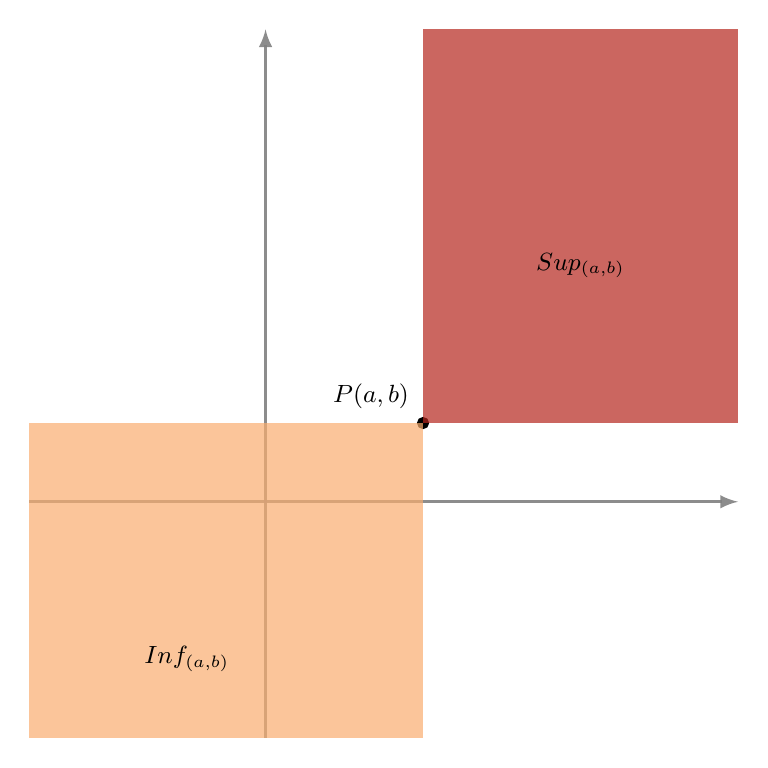
\begin{tikzpicture}[scale=1, >=latex]
    \draw[very thick, gray, opacity=0.9,->] (-3,0)--(6,0);
    \draw[very thick, gray, opacity=0.9,->] (0,-3)--(0,6);
    \node[draw, circle,fill, minimum width=4pt, inner sep=0pt,
        label=above left:{\small$P(a,b)$}](P) at (2,1){};
    \fill[BrickRed,opacity=0.7] (2,1) rectangle (6,6);
    \fill[Apricot,opacity=0.7] (2,1) rectangle (-3,-3);
    \node at (4,3) {\small$Sup_{(a,b)}$};
    \node at (-1,-2) {\small$Inf_{(a,b)}$};
\end{tikzpicture}
\end{center}
\caption{Illustration des éléments supérieurs et inférieurs d'un point $(a,b)$
par la relation $\mathcal{R}$}%
\label{fig:point_sup}
\end{figure}

\item Cette relation est elle totale.

    D'après le graphique on peut observer que pour un point $(a,b)$, on ne peut
    pas le comparer à tous les points. Par exemple si considère le point
    $P(0,0)$ et le point $Q(-1,1)$, Ils ne sont pas comparables.
    
\end{enumerate}
% }}} Relation d'ordre %
% Vérficiation groupe {{{ %
\section{Vérification groupe}%
\label{sec:vérification_groupe}
Soit $G=\mathbb{R}\times \mathbb{R}^{*}$ et la loi $*$ définie comme suit:

\begin{equation}
    (x_1,y_1) * (x_2, y_2) = (x_2y_1 + \frac{x_1}{y_2}\;,\; y_1y_2)
\end{equation}

\begin{description}
    \item[Loi interne]:
        Soit $P_1=(x_1,y_1),\;P_2=(x_2,y_1) \in G$, montrons que $P_1\;*\;
        P_2\in G$

        On a $ x_2 \text{ et } x_2\in \mathbb{R}$  et $y_1 \text{ et } y_2\in
        \mathbb{R}^{*}\implies$

        \begin{equation*}
            \left\{\begin{array}{lll}
                    x_2y_1 +\frac{x_1}{y_2}&\in& \mathbb{R}\\[4pt]
                    y_1y_2 & \in & \mathbb{R}^{*}
                \end{array}\right.
        \end{equation*}
        Donc $$P_1 \;*\;P_2 \in G$$

    \item [Associative, commutative]
        Soient $P_i=(x_i,y_i)\; i\in\{1,2,3\}$ trois points de $G$.
        \begin{itemize}
            \item Calculons la valeur de $(P_1\;*\;P_2)\;*\;P_3$
            \begin{eqnarray}
                (P_1\;*\;P_2)\;*\;P_3  &=& (x_3y_1y_2 + \frac{x_2y_1 +
                \frac{x_1}{y_2}}{y_3}\;,\; y_1y_2y_3) \\
                    P_1\;*(P_2\;*\;P_3)  &=& \big((x_3y_2+\frac{x_2}{y_3})y_1 +
                    \frac{x_1}{y_2y_3}\;,\; y_1y_2y_3\big)
            \end{eqnarray}
            Ce qui prouve qu'on possède l'égalité entre les deux expressions.
        \end{itemize}

        \textbf{Commutative}?
        Il suffit de calculer par exemple
        $$
        (1, 4)\;*\;(3,1) = (12 + 1 ,4)\neq (3+\frac{3}{4},4) = (3,1)\;*\;(1,4)
        $$
        Donc la loi n'est pas \textbf{commutative}.

    \item[Élément neutre]:

        Soit $P=(x,y)$, cherchons un élément $E=(e_1,e_2)$ 
        tel que
        \begin{equation}
            P \;*\; E = P\quad \forall P\in\mathbb{R}^2
        \end{equation}
        On obtient que:

        \begin{equation}
            \left\{
            \begin{array}{ccc}
                e_1y + \dfrac{x}{e_2} &=& x\\[4pt]
                y e_2 &=& y
        \end{array}\right.
        \implies 
            \left\{
            \begin{array}{ccc}
                e_1y&=& 0\\[4pt]
                e_2 &=& 1
        \end{array}\right.
\;\;
            \left\{
            \begin{array}{ccc}
                e_1&=& 0\\[4pt]
                e_2 &=& 1
        \end{array}\right.
        \end{equation}
        Puisque la loi n'est pas commutative, il faut aussi vérifier 
        $$
        (0,1)\;*\; (x,y) = (x,y) \quad\forall (x,y)\in\mathbb{R}^2
        $$

        On as 
        $$(0,1)\;*\; (x,y) = (x + \frac{0}{y}\;,\; y) = (x,y)
        $$

        Donc G admet un élément neutre $E(0,1)$.

    \item[Groupe]: Pour que $G$ soit un groupe, il faut que chaque élément de
        $G$ admet un opposé.

        Donc soit $P=(x,y)\in G$, cherchons $P^{'}=(x^{'}, y^{'})\in G$ tel que

        \begin{equation}
            P\;*P^{'} = P^{'}\;*\; P = (0,1)
        \end{equation}

        Si on applique la première relation $P\;*\; P^{'}$, on aura alors que:

$$
            \left\{
            \begin{array}{ccc}
                x^{'}y + \frac{x}{y^{'}}&=& 0\\[4pt]
                yy^{'}&=& 1
        \end{array}\right.
        \implies
            \left\{
            \begin{array}{ccc}
                (x^{'} + x)y&=& 0\\[4pt]
                y^{'}&=& \dfrac{1}{y}
        \end{array}\right.
        \implies
            \left\{
            \begin{array}{ccc}
                x^{'}  &=& -x\\[4pt]
                y^{'}&=& \dfrac{1}{y}
        \end{array}\right.
$$
On doit vérifier maintenant que $P^{'}=(-x,\frac{1}{y}$, vérifie aussi
$P^{'}\;*\;P$

\begin{equation}
    (-x,\frac{1}{y}) \;*\; (x,y) = (\frac{x}{y} - \frac{x}{y}, \frac{y}{y}) =
    (0,1) 
\end{equation}
Donc chaque élément $(x,y)$ admet un opposé $(-x, \frac{1}{y})$. Ainsi on conclut
que $(G, *)$ est un groupe non abélien.
\end{description}
% }}} Vérficiation groupe %
% Automorphisme antérieur {{{ %
\section{Automorphisme antérieur}%
\label{sec:automorphisme_antérieur}

Soit $(G,.)$ un groupe. Pour chaque élément  $a\in G$, on note la fonction
$\tau_a$ définie comme suit:

\begin{equation}
    \label{eq:automorphism}
    \tau_a:\left\{\begin{array}{lll}
            G &\longrightarrow & G\\
            x & \longrightarrow & a^{-1}.x.a
        \end{array}
    \right.
\end{equation}

\begin{description}
    \item[Morphisme du groupe]:

        Soit deux éléments $x$ et $y$ dans $G$
        On a :
        \begin{eqnarray}
            \tau_a\big(x.y\big) &=& a^{-1}.x.y.a\\[4pt]
                                &=&
                                \underbrace{a^{-1}x.a}_{\tau_a(x)}.\underbrace{a^{-1}.y.a}_{\tau_a(y)}\\[4pt]
                                & = & \tau_a(x).\tau_a(y)
        \end{eqnarray}
        Ce qui prouve que $\tau_a$ est un morphisme de groupe.

    \item[Composée]: 
        \begin{equation}
            \forall a,b\in G, \quad \tau_a\circ \tau_b =\tau_{b.a} 
        \end{equation}

        On a:

        \begin{eqnarray}
            \tau_a\circ\tau_b(x) &=&\tau_a\big(\tau_b(x)\big) \\[4pt]
                                 &=& \tau_a\big(b^{-1}.x.b\big)\\
                                 &=& a^{-1}.b^{-1}.x.b.a\\
                                 &=& (b.a)^{-1}.x.(b.a)\\
                                 &=& \tau_{b.a}(x)\label{eq:compose}
        \end{eqnarray}
    \item[Bijection]: Soit $a\in G$, montrons que l'application est $\tau_a$
        est bijective.\\

        Puisque $(G,.)$ est un groupe, chaque élément $a$ admet un opposé qu'on
        note $a^{-1}$. Selon l'équation~\eqref{eq:compose}, on a

        \begin{equation}
            \tau_a\circ\tau_{a^{-1}}= \tau_{a^{-1}.a}=\tau_e=\text{Id}_G
        \end{equation}

De même on a:

        \begin{equation}
            \tau_{a^{-1}}\circ\tau_{a}= \tau_{a.a^{-1}}=\tau_e=\text{Id}_G
        \end{equation}
        Ainsi chaque application $\tau_a$ est bijective et son inverse est
        $\tau_{a^{-1}}$.
    \item[Groupe des morphisme]:
        On note $\Theta=\left\{\tau_a\;|\; a\in G\right\}$, montrons qu
        e$(\Theta, \circ)$ est un sous groupe du groupe des fonctions de $G$
        vers $G$.

    \begin{itemize}
        \item  \textbf{Elément neutre}: On a $\tau_{e}: x \rightarrow e^{-1}.x.e=x$
            Ainsi $$\tau_e = \text{Id} \in \Theta$$
        \item \textbf{Loi interne} : Selon la question (b), on a:
            $$
            \tau_a \circ \tau_b = \tau_{b.a}  \in \Theta
            $$

        \item \textbf{Opposé}: Selon la question (c), on a
            $$
             \forall a\in G \tau_a\circ\tau_{a^{-1}} =
            \tau_{a^{-1}}\circ\tau{a}= \text{id}
            $$

Donc chaque élément admet un opposé.
Ainsii que $\Theta$ un \textbf{groupe}.
    \end{itemize}


\end{description}
% }}} Automorphisme antérieur %
% Polynomes {{{ %
\section{Polynômes}%
\label{sec:polynomes}

Soient $P= 2x^4 + 2x^3 -2x -2$ et $Q=-x^4 + 1$ deux polynômes dans $\mathbb{R}[X]$

\begin{enumerate}
    \item Déterminer le \textbf{PGCD}(P,Q):\\

        \polylonggcd{2x^4+2x^3-2x-2}{-x^4+1}\\

        Ainsi on conclut que le $D=(X^2-1)$, puisque le PGCD doit être
        \textbf{unitaire}.

\item Démontrer que $x^3-x$ est un multiple de $D$.\\

    \polylongdiv[style=B]{x^3-x}{x^2-1}

\item Pour retrouver alors $U$ et $V$, on  détermine les polynômes de
    \textbf{Bézout} puis on multiplie par $x$. 

    Selon la deuxième equation de la décomposition on trouve que 

    \begin{eqnarray}
        Q &=& (2x^3-2x)(-\frac{1}{2}x) - D\\
        D &=& -Q + (\frac{1}{2}x)(2x^3-2x)
    \end{eqnarray}
    On remplace maintenant $(2x^3-2)$ par son expression dans la première
    equation

    \begin{eqnarray}
        D &=& -Q+ (\frac{1}{2}x)(P + 2Q)\\
        D &=& \frac{1}{2}x P + (x-1)Q
    \end{eqnarray}
Finalement pour retrouver $C$ il suffit de multiplier par $x$
\begin{equation}
    C = xD = \underbrace{\big(\frac{1}{2}x^2\big)}_{U}P +
    \underbrace{\big(x^2-x\big)}_{V}Q
\end{equation}
\end{enumerate}

% }}} Polynomes %

\end{document}
